\section{Auswertung}
\label{sec:Auswertung}
Die in dieser Auswertung erstellten Plots werden mithilfe der \textit{Python}-Erweiterung 
\textit{matplotlib}~\cite{matplotlib} erstellt. Die Fortplanzung der Messunsicherheiten werden mithilfe von
\textit{uncertainties}~\cite{uncertainties} bestimmt und genügen der Gaußschen Fehlerfortplanzung
\begin{equation*}
    \symup{\Delta} F = \sqrt{\sum_{i}\left(\frac{\symup{d}F}{\symup{d}y_{i}}\symup{\Delta} y_{i} \right)^2}.
\end{equation*}
Die Messunsicherheiten der Zählraten $N$ sind poissonverteilt und werden daher mit $\symup{\Delta}N = \sqrt{N}$ berechnet.

\subsection{Charakteristik des GMZ}

\begin{figure}[H]
    \centering
    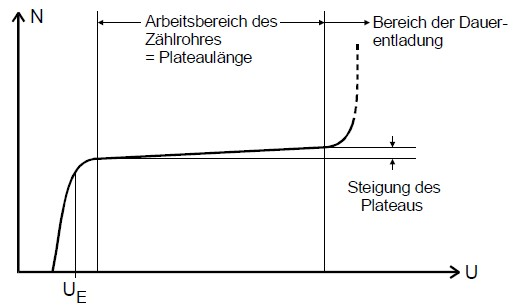
\includegraphics{build/charakteristik.pdf}
    \caption{Graphische Darstellung der Charakteristik des GMZ mit eingezeichneter Ausgleichsgerade der %
    Messwerte des Plateaus.}
    \label{fig:charakteristik}
\end{figure}

\begin{longtable}{c c c}
    \caption{Messwerte zur Bestimmung der Charakteristik des GMZ sowie der freigesetzten Ladung.} \label{tab:messdaten} \\
    \hline
    {1} & {2} & {3} \\
    \hline
    \endfirsthead
    \caption[]{Messwerte zur Bestimmung der Charakteristik des GMZ sowie der freigesetzten Ladung. (Fortsetzung)}\\
    \hline
    \endhead
    \hline
    \endfoot
    2 & 3 & 4 \\
    \bottomrule
\end{longtable}



\subsection{Freigesetzte Ladung im GMZ}



\begin{figure}[H]
    \centering
    \includegraphics{build/ladung.pdf}
    \caption{Darstellung der für bestimmte Spannungen freigesetzten Ladungen im GMZ.}
    \label{fig:ladung}
\end{figure}